%%
%% Copyright 2007, 2008, 2009 Elsevier Ltd
%%
%% This file is part of the 'Elsarticle Bundle'.
%% ---------------------------------------------
%%
%% It may be distributed under the conditions of the LaTeX Project Public
%% License, either version 1.2 of this license or (at your option) any
%% later version.  The latest version of this license is in
%%    http://www.latex-project.org/lppl.txt
%% and version 1.2 or later is part of all distributions of LaTeX
%% version 1999/12/01 or later.
%%
%% The list of all files belonging to the 'Elsarticle Bundle' is
%% given in the file `manifest.txt'.
%%

%% Template article for Elsevier's document class `elsarticle'
%% with harvard style bibliographic references
%% SP 2008/03/01
%%
%%
%%
%% $Id: elsarticle-template-harv.tex 4 2009-10-24 08:22:58Z rishi $
%%
%%
\documentclass[preprint,authoryear,12pt]{elsarticle}

%% Use the option review to obtain double line spacing
%% \documentclass[authoryear,preprint,review,12pt]{elsarticle}

%% Use the options 1p,twocolumn; 3p; 3p,twocolumn; 5p; or 5p,twocolumn
%% for a journal layout:
%% \documentclass[final,authoryear,1p,times]{elsarticle}
%% \documentclass[final,authoryear,1p,times,twocolumn]{elsarticle}
%% \documentclass[final,authoryear,3p,times]{elsarticle}
%% \documentclass[final,authoryear,3p,times,twocolumn]{elsarticle}
%% \documentclass[final,authoryear,5p,times]{elsarticle}
%% \documentclass[final,authoryear,5p,times,twocolumn]{elsarticle}

%% if you use PostScript figures in your article
%% use the graphics package for simple commands
%% \usepackage{graphics}
%% or use the graphicx package for more complicated commands
%% \usepackage{graphicx}
%% or use the epsfig package if you prefer to use the old commands
%% \usepackage{epsfig}

%% The amssymb package provides various useful mathematical symbols
\usepackage{graphicx}
\usepackage{epstopdf}
\usepackage{amssymb}
\usepackage{amsmath}
\usepackage{a4wide}
\usepackage{color}
%\usepackage{subcaption}
\newcommand{\hilight}[1]{\colorbox{yellow}{#1}}
%% The amsthm package provides extended theorem environments
%% \usepackage{amsthm}
\newcommand\solidrule[1][1cm]{\rule[0.5ex]{#1}{1pt}}
\newcommand\dashedrule{\mbox{\solidrule[1mm]\hspace{1mm}\solidrule[1mm]\hspace{1mm}\solidrule[1mm]\hspace{1mm}}}
\newcommand{\ustar}{\ensuremath{U^{*}}}

%% The lineno packages adds line numbers. Start line numbering with
%% \begin{linenumbers}, end it with \end{linenumbers}. Or switch it on
%% for the whole article with \linenumbers after \end{frontmatter}.
%% \usepackage{lineno}

%% natbib.sty is loaded by default. However, natbib options can be
%% provided with \biboptions{...} command. Following options are
%% valid:

%%   round  -  round parentheses are used (default)
%%   square -  square brackets are used   [option]
%%   curly  -  curly braces are used      {option}
%%   angle  -  angle brackets are used    <option>
%%   semicolon  -  multiple citations separated by semi-colon (default)
%%   colon  - same as semicolon, an earlier confusion
%%   comma  -  separated by comma
%%   authoryear - selects author-year citations (default)
%%   numbers-  selects numerical citations
%%   super  -  numerical citations as superscripts
%%   sort   -  sorts multiple citations according to order in ref. list
%%   sort&compress   -  like sort, but also compresses numerical citations
%%   compress - compresses without sorting
%%   longnamesfirst  -  makes first citation full author list
%%
%% \biboptions{longnamesfirst,comma}

% \biboptions{}

\journal{Journal of Fluid Structures}

\begin{document}
\begin{frontmatter}

%% Title, authors and addresses

%% use the tnoteref command within \title for footnotes;
%% use the tnotetext command for the associated footnote;
%% use the fnref command within \author or \address for footnotes;
%% use the fntext command for the associated footnote;
%% use the corref command within \author for corresponding author footnotes;
%% use the cortext command for the associated footnote;
%% use the ead command for the email address,
%% and the form \ead[url] for the home page:
%%
%% \title{Title\tnoteref{label1}}
%% \tnotetext[label1]{}
%% \author{Name\corref{cor1}\fnref{label2}}
%% \ead{email address}
%% \ead[url]{home page}
%% \fntext[label2]{}
%% \cortext[cor1]{}
%% \address{Address\fnref{label3}}
%% \fntext[label3]{}

\title{}

%% use optional labels to link authors explicitly to addresses:
%% \author[label1,label2]{<author name>}
%% \address[label1]{<address>}
%% \address[label2]{<address>}

\author{}

\address{}

\begin{abstract}
%% Text of abstract

\end{abstract}

\begin{keyword}
%% keywords here, in the form: keyword \sep keyword

%% MSC codes here, in the form: \MSC code \sep code
%% or \MSC[2008] code \sep code (2000 is the default)

\end{keyword}

\end{frontmatter}

% \linenumbers

%% main text
\section{Introduction} 

The search for alternate energy sources which could be categorised  under the "green" label has become important area of research in the modern word. Solar, wind power and wave power are some of the examples of these sources.  Recently,a new branch of research has been developing to extract energy from flow induced vibrations(\cite{Bernitsas2008a-concept}). It has been hypothesized that this technique may work efficiently in areas where regular turbines cannot. 

A simple structure that is susceptible to flow-induced vibrations that are suitable for energy extraction are slender structures,such as cylinders, elastically mounted perpendicular to a fluid stream. With regards to a slender body two common types of   flow induced vibrations are Vortex Induced Vibrations (VIV) and aeroelastic galloping. Significant research has been carried out by Bernitsas and his team on extracting useful energy from VIV. Some of their significant work includes investigating the influence  of physical parameters such as mass ratio (the ratio of the mass of the cylinder and the displaced fluid), Reynolds number, mechanical properties(\cite{Raghavan2010a} ,\cite{Lee2011b}) and location (effect of the bottom boundary) (\cite{Raghavan2009}). However,the possibility of extracting energy using aeroelastic galloping has not been thoroughly investigated. Some theoretical work was carried out by (\cite{Barrero-Gil2010a}). Utilizing galloping may be a more viable method to harness energy from flow induced vibrations as it is not bounded by a "lock-in" range of reduced velocities(ratio between the freestream velocity and the product of the natural frequency of the system and the characteristic length).Therefore it is preferable to investigate further the possibility of harnessing energy from flow induced vibrations using aeroelastic galloping.

Real life energy harvesting systems use high damping ratios where the energy generator (e.g electrical generator) puts a significant amount of damping into the system. Therefore it is crucial to investigate  the behaviour of aeroleastic galloping scenarios at high damping ratios in order to optimise the system to obtain a acceptable power output.Hence the focus of this paper is concentrated on investigating the mechanical power output of high-damped galloping systems in laminar flow.

According to \cite{Paidoussis2010},\cite{Glauert1919} has provided a criterion for galloping by considering the auto-rotation of an aerofoil.  \cite{DenHartog1956}  has provided a theoretical explanation for galloping for iced electric transmission lines. A non-linear theoretical aeroelastic model to predict the response of galloping was developed by \cite{Parkinson1964} based on the quasi-steady state (QSS) theory. Experimental lift and drag data on a fixed square prism at different angles of attack were used as an input for the theoretical model. It essentially used a curve fit of the transverse force to predict the galloping response. The study managed to achieve a good agreement with experimental (wind tunnel) data.\cite{Joly2012} have observed that finite element simulations shows a sudden change in amplitudes  below a critical values of the mass ratio, which the  (QSS) model fails to reproduce. The Parkinson's equation was essentially modified to account for the vortex shedding and managed to produce the effects to the amplitude at low mass ratios.
\cite{Barrero-Gil2010a} have investigated the possibility of extracting power from vibrations caused by galloping using quasi-steady state theory. In the conclusions of that paper it was pointed out that in order to obtain a high power to area ratio the mass-damping ($m^*\zeta$) parameter should be kept low as well as the frequency of oscillations should be carefully matched \hilight{have a good agreement with the size of the cross section}. Another interesting conclusion was that energy conversion systems which uses galloping could operate over  a large range of flow velocities unlike VIV energy harvesting systems where the factor of energy conversion has a strong dependence on the incoming flow velocity. 
\textbf{Nomenclature}



\begin{tabular}{ll}
$a_1,a_3,a_5,a_7$ & coefficients of the polynomial to determine $C_y$ \\ 
$C_y$ & instantaneous lift \\
$F_y$ & force due to $C_y$  \\ 
$\rho$ & fluid density  \\
$m$ & mass of the body \\
$m_a$ & added mass \\
$c$ & damping constant/damping factor \\
$k$ & spring constant \\
$U_i$ & induced velocity \\
$\theta$ & induced angle of incidence \\
$U$ & freestream velocity \\
$y,\dot{y},\ddot{y}$ & transverse displacement, velocity and acceleration   \\
$A$ & displacement amplitude\\
$\mathcal{A}$ & cross sectional area\\ 
$F_0$& force due to shedding \\
$\omega_s$& vortex shedding frequency \\
$t$ & time \\
$P_{mean}$& mean power \\
$f=\frac{1}{2\pi}\sqrt{\frac{k}{m}}$& natural frequency of the system \\
$\omega_n= 2 \pi f$& natural frequency of the system  \\
$D$ & characteristic length of the body  \\
$m^*=\frac{m}{\rho \times \text{Volume of the body}}$& mass ratio \\
$U^*=\frac{U}{f \times D}$& reduced velocity  \\
$\zeta= \frac{c}{2 m \omega_n}$& damping ratio \\
$P_t$   & power transferred to the body by the fluid \\
$P_d$& power dissipated due to mechanical damping  \\
$Re$& Reynolds number  \\
$\theta= \tan^{-1}{(\frac{\dot{y}}{U})}$& instantaneous angle \\
& \\
& \\
\end{tabular}  

\section{Background theory}

\subsection{Mathematical model (Quasi-steady )}

 One of the widely used mathematical model to predict the system response under galloping is the Quasi-steady state (QSS) model, incorporated by \cite{Parkinson1964} for a square cross section. The equation of motion of the body under galloping is given by Eq. \eqref{equationofmotion}. The forcing term $F_y$ is given by Eq.\eqref{lift equation}.
 
 \begin{figure}
\setlength{\unitlength}{\textwidth}

  \begin{picture}(1,0.23)(0,0.74)
    
  \put(0.2,0.76){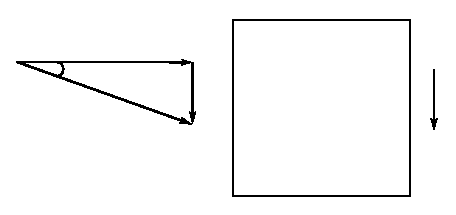
\includegraphics[width=0.5\unitlength]{../FnP/gnuplot/setup-1.eps}}         
      
      
   
 	\put(0.315,0.93){$U$}
 	\put(0.3,0.84){$U_i$}
    \put(0.42,0.88){$\dot{y}$}
    \put(0.28,0.895){ $\theta$}
    \put(0.7,0.87){\small $(+)$}
      	

 	
 	 

     

  \end{picture}

 \caption{Induced angle of attack on the square prism due to the resultant of free-stream velocity of the fluid and transverse velocity of the body.}
    \label{fig:setup_1}
\end{figure}

\begin{equation}
\label{equationofmotion}
(m+m_a)\ddot{y}+c\dot{y}+ky=F_y
\end{equation}

\begin{equation}
\label{lift equation}
F_y=\frac{1}{2}\rho U^2\mathcal{A}C_y
\end{equation}

 In the QSS  model $C_y$ is determined by an interpolating polynomial based on the stationary lift and drag data. The order of the interpolation polynomial has varied from study to study. For  example a $7^{th}$ polynomial order was used in \cite{Parkinson1964} and $3^{rd}$ order polynomial was used in \cite{Barrero-Gil2009}. \cite{Ng2005} concluded that using a $7^{th}$ order polynomial is sufficient and a polynomial higher than that of $7^{th}$ order polynomial neither provides a significantly better result nor does it exhibit an additional amplitudes of oscillation. Thus a $7 ^{th}$ order interpolating polynomial was incorporated in this present study. 

\begin{equation}
\label{cy ploynomial}
C_y(\theta)=a_1\left(\frac{\dot{y}}{U}\right)+a_3\left(\frac{\dot{y}}{U}\right)^3+a_5\left(\frac{\dot{y}}{U}\right)^5+a_7\left(\frac{\dot{y}}{U}\right)^7
\end{equation}

%\begin{equation}
%\label{modified_equation_of_motion}
%\ddot{y}+c^*\dot{y}+k^*y=\frac{1}{2}\rho U^2A
%\end{equation}

\cite{Joly2012} reported a reduction of displacement amplitude at low mass ratios. Therefore in order to account for it a sinusoidal forcing function to the RHS of the oscillator model (Eq. \eqref{equationofmotion})was introduced, in order to represent forcing due to VIV. This method provided satisfactory results with the numerical simulations obtained at low mass ratios. In this study, the forcing due to VIV is incorporated using a sinusoidal forcing function $F_0\sin{\omega_{s}t}$ added to the RHS of the equation. $\omega_{s}$ and $F_0$ represents shedding frequency and the maximum force due to shedding respectively. Thus, the final equation is given by Eq. \eqref{final_equation_motion}.    

\begin{equation}
\label{final_equation_motion}
(m{+}m_a)\ddot{y}{+}c{+}\dot{y}{+}ky{=}\frac{1}{2}\rho U^2 \mathcal  {A} \Bigg(a_1\left(\frac{\dot{y}}{U}\right){+}a_3\left(\frac{\dot{y}}{U}\right)^3{+}a_5\left(\frac{\dot{y}}{U}\right)^5{+}a_7\left(\frac{\dot{y}}{U}\right)^7 \Bigg){+} F_0\sin{(\omega_s t)}
\end{equation}

This equation could be solved by time integration methods. In  this study  `Ode 45' routine in MATLAB was used to obtain the solutions.

\subsection{Calculation of average power}

 The dissipated power due to the mechanical damping could be expressed as the harvested power output assuming that the other  power dissipation due to internal damping such as friction of the system is negligible. Therefore the mean power output could be given by Eq. \eqref{power}. 
  
 
 \begin{equation}
 \label{power}
P_{mean}=\frac{1}{T}\int_{0}^{T}(c\dot{y})\dot{y} dt
 \end{equation}
 
 \begin{figure}

  \setlength{\unitlength}{\textwidth}
  \begin{picture}(1,0.25)(0,0.8)
  
    % % %90
      \put(0.025,0.81){\includegraphics[width=0.5\unitlength]{../FnP/gnuplot/lift_curve_165.eps}}
      \put(0.495,0.81){\includegraphics[width=0.5\unitlength]{../FnP/gnuplot/lift_curve_park.eps}}
 	\put(0.02,0.93){ \large $C_y$} 	
% 	\put(0.56,1.02){ $\theta$}
 	
        \put(0.25,0.8){ $\theta$} 	
        \put(0.75,0.8){ $\theta$}
        
        \put(0.105,1.01){(a)}
        \put(0.565,1.01){(b)}
      \end{picture}

  \caption{Lift coefficient, $C_y$ \JL{$C_y$ is upper case here, lower case on the figure. Make them match what is in the nomenclature}, as a function of incidence angle $\theta$, for a static square cross section. (a) Data from simulations at $Re=165$  (b) data from \cite{Parkinson1964} at $Re=22300$. Points ($\bullet$) are measurements from the simulations. The solid lines in both plots are 7th-order interpolating polynomial used to predict the fluid forcing for the QSS model.}
    \label{fig:lift_curves}
\end{figure}
 \vspace{20mm}
 \begin{table}[ht]

\begin{center}
\setlength{\unitlength}{\textwidth}

\begin{tabular}{c c c c c} % centered columns (4 columns)
\hline\hline %inserts double horizontal lines
\\[0.2ex]
Case & $a_1$ & $a_3$ & $a_5$ & $a_7$ \\ [0.8ex] % inserts table 
%heading
\hline 
\\[0.8ex]% inserts single horizontal line
Re=165 & 1.3 & 125.3 & 1825.73 & 8765.3 \\[0.8ex] % inserting body of the table
Re=22300 & 2.69 & 168 & 1670 & 59900 \\ [1ex] % [1ex] adds vertical space
\hline %inserts single line
\end{tabular}

\caption{Coefficient values used in the 7th order interpolation polynomial for high ($Re=165$) and low ($Re=22300$) Reynolds numbers. These data are used as input data to calculate the RHS of Eq.\ref{final_equation_motion} throughout this study.}
 
\label{table:nonlin} % is used to refer this table in the text
\end{center}
\end{table}


 
\subsection{Parameters used} 
 
The stationary data and the fluid-structure interaction (FSI) data were obtained using a higher order spectral element code which simulate 2D laminar flow. The Reynolds number was kept at 165 as it was pointed out by \cite{Sheard2009} and \cite{Tong2008} that the 3 dimensional transition for a square cylinder occurs at approximately Re=160. $F_0$ was kept at $0.4937$ which was obtained by using a simple linear interpolation on the data presented in \cite{Joly2012}. $\omega_s$ was set to $0.98$ winch was obtained by performing a power spectral analysis of the stationary data at $0^0$. Stationary $C_y$ data were obtained at different angles of attack ranging from $0^0$ to $16^0$. The average power was obtained by using Eq. \eqref{power} with data sets consisting substantial amount of peaks. Power data  at Re=22300 were obtained using input $C_y$ data in \cite{Parkinson1964} in order to provide a comparison between high and low Reynolds numbers. $m^*$ was kept at 1163 for \reynoldsnumber=22300 (Similar as \cite{Parkinson1964}) and $m^*=20$ for \reynoldsnumber=165. These parameters  were used throughout this study unless otherwise specified. 


 FSI data were obtained for the oscillating (free-vibration) scenario. The Naiver-Stokes equations were solved using an accelerated frame of reference using the previously mentioned code. A three-step time splitting scheme together with high-order Lagrangian polynomials were used to obtain the solution. The details of the method could be found in \cite{Thompson2006,Thompson1996a}. This code was incorporated in \cite{Leontini2011,Leontini2007a}  where it was employed in a fluid-structure interaction problems. 
 
 The computational domain consists of 690 quadrilateral macro elements where majority of the elements were concentrated near the square section. A freestream condition was given to the inlet, top and bottom boundaries and the normal velocity gradient was set to zero at the outlet. A convergence study was performed by changing the order of the polynomial ($p$-refinement) at $U^*=40$ and Re $165$. A 9th order polynomial together with a time step of $\frac{\Delta tU}{D}=0.001$ was sufficient to ensure an accuracy of $2\%$ with regards to amplitude of oscillation.  
 

 
 
 

 
 
 
 











\section{Results}
\begin{figure}
  \setlength{\unitlength}{\textwidth}

  \begin{picture}(1,0.72)
%(0,0.35)
    
    % % %Parkinson Data 
    \put(0.025,0.48){\includegraphics[width=0.5\unitlength]{../FnP/gnuplot/displacement_amp_re_parkinson_1.eps}}
    \put(0.025,0.25){\includegraphics[width=0.5\unitlength]{../FnP/gnuplot/velocity_amp_re_parkinson.eps}}
    \put(0.025,0.02){\includegraphics[width=0.5\unitlength]{../FnP/gnuplot/mean_power_re_parkinson.eps}}
    
    % Re 165 Data 
    \put(0.495,0.48){\includegraphics[width=0.5\unitlength]{../FnP/gnuplot/displacement_amp_re165.eps}}
    \put(0.495,0.25){\includegraphics[width=0.5\unitlength]{../FnP/gnuplot/velocity_amp_re165.eps}}
    \put(0.495,0.02){\includegraphics[width=0.5\unitlength]{../FnP/gnuplot/mean_power_re_165.eps}}
   
%    \put(0.25,0.93){\ustar}
%    \put(0.8,0.93){\ustar}
%    \put(0.25,0.63){\ustar}
%   \put(0.8,0.63){\ustar}
    \put(0.25,0.0){\ustar}
    \put(0.75,0.0){\ustar}
    
    \put(0.00,0.685){$\frac{A}{D}$}
%    \put(0.52,1.075){$\frac{A}{D}$}
    \put(0.00,0.44){$\frac{V}{D}$}
%    \put(0.52,0.83){$\frac{V}{D}$}
    \put(-0.01,0.15){$\frac{P_{m}}{\rho \mathcal{A}U^3 }$}
%    \put(0.5,0.54){$\frac{P_{m}}{\rho \mathcal{A}U^3 }$}
    
    \put(0.085,0.685){\small(a)}
    \put(0.555,0.685){\small(b)}
    \put(0.085,0.455){\small(c)}
    \put(0.555,0.455){\small(d)}
    \put(0.085,0.225){\small(e)}
    \put(0.555,0.225){\small(f)}   
  \end{picture}

%  \vspace{-4cm}
  \caption{Velocity and displacement amplitude and mean power  as a function of $U^*$. (a), (c) and (e) are calculated using input $C_y$ data at $Re=22300$ obtained by \cite{Parkinson1964} at three different damping ratios: $\zeta=0.0125$ (\ding{83}), $\zeta=0.015$ (\ding{116}) and $\zeta=0.0175$ (\ding{108}). (b),(d) and (f) are from $C_y$ data at $Re=165$ and are calculated  from the fixed body simulations at three different  different damping ratios: $\zeta=0.075$ ($\times$), $\zeta=0.1$ (\ding{117}) and $\zeta=0.15$ (+). The multiple branches for the higher Re are due to the hysteresis between two solutions.}
  
  \label{fig:uncollapsed_data}
\end{figure}




\subsection{Displacement,velocity and power output as a function of reduced velocity}


 The quasi-steady analysis data reveals that the displacement amplitude tend to grow with increasing $U^*$ Fig.\ref{fig:uncollapsed_data} (a) and (b). The onset of galloping is delayed with increasing $\zeta$ for both high and low Reynolds numbers. This echo the findings of previous studies \cite{Parkinson1964} and \cite{Barrero-Gil2010a}. Hysteresis could be observed at higher Reynolds numbers. 

 
 \subsubsection*{Power vs $U^*$}
 
 The mean power grows, peaks and then reduces as $U^*$ is increased (Fig.\ref{fig:uncollapsed_data} (e) and (f)) for each value of $\zeta$. A shift of the peak power could be observed as $\zeta$ increases. However, the magnitude of the peaks remain constant for all the values of $\zeta$. A similar observation could be made from the results of \cite{Barrero-Gil2010a}. It could be observed that unlike VIV the  system has no preferred frequency. The onset of galloping and the peak power occurs at different $U^*$ at when the damping ratio is changed. The peak power remains constant regardless of $U^*$.
 
 \subsection{Galloping response and natural frequency}
 
 If the oscillator equation Eq.\eqref{final_equation_motion} is considered from a power perspective (disregarding the shedding term as the net effect is negligible as system oscillates at natural frequency which is far from shedding frequency), it could be seen that the forcing term on RHS of the equation is only dependent on transverse velocity($\dot{y}$) which is essentially the input power of the system. On the RHS, the mechanical damping or system damping is the only term that takes out power at any instant by the product of damping force and the velocity ($P_d$). The inertia and the stiffness terms governs the frequency of the system but the forces associated by those terms are conservative forces i.e there is zero net energy in or out of the system when averaged over a period. Therefore it appears that the system is governed by the transverse velocity rather than the natural frequency.
 

 Using $U^*$ and $\zeta$ assumes that the system has a preferred frequency. The effect of fixing $\zeta$ and increasing $U^*$ actually decreases damping constant for a fixed free-stream velocity.($U^*=\frac{U}{f \times D}$, $\zeta= \frac{c}{2 m \omega_n}$ ). Both these effects leads to the multiple lines that are horizontally transpose when $\zeta$ is increased(Fig.\ref{fig:uncollapsed_data} (e) and (f)). Therefore the effect of $\zeta$ essentially scales up the damping coefficient for a fixed $U^*$. 
 \vspace{1cm}
 
 Therefore a single set of results for a given instantaneous lift ($C_y$) could be obtained if we were to plot displacement, velocity and power as a function of damping constant $c$ (Fig \ref{fig:collpased_data} (a),(b),(c) and (d)). A similar maximum velocity could be obtained for a given `c'. Fig.\ref{fig:same_max_vel} clearly shows the validity of this argument. 
 

\begin{figure}
  \setlength{\unitlength}{\textwidth}
       
        \begin{picture}(1,0.52)

      % % % Parkinson Data 
      \put(0.025,0.27){\includegraphics[width=0.5\unitlength]{../FnP/gnuplot/velocity_amp_collapsed_parkinson.eps}}
      \put(0.495,0.27){\includegraphics[width=0.5\unitlength]{../FnP/gnuplot/velocity_amp_collapsed_re165.eps}}
      
      \put(0.025,0.02){\includegraphics[width=0.5\unitlength]{../FnP/gnuplot/mean_power_collapsed_parkinson.eps}}
      \put(0.495,0.02){\includegraphics[width=0.5\unitlength]{../FnP/gnuplot/mean_power_collapsed_re_165.eps}}
      
      
      \put(0.23,0.00){ $c\rho\mathcal{A}U$}
      \put(0.73,0.00){ $c\rho\mathcal{A}U$}
      
      \put(0.01,0.405){$\frac{V}{D}$}
      
      \put(0,0.13){$\frac{P_{m}}{\rho \mathcal{A}U^3 }$}
      \put(0.085,0.475){\small(a)}
      \put(0.555,0.475){\small(b)}
      \put(0.095,0.225){\small(c)}
      \put(0.555,0.225){\small(d)}
      
    \end{picture}

  \caption{ Velocity amplitude and mean power  as a function of $c$ (damping constant). (a) and (c)  are calculated using input $C_y$ data at Re=22300 obtained by \cite{Parkinson1964} and present data at three different damping ratios: $\zeta=0.0125$ (\ding{83}), $\zeta=0.015$ (\ding{116}) and $\zeta=0.0175$ (\ding{108}). (b)and (d)  are at Re=165 are calculated  from the fixed body simulations and present data from three different damping ratios: $\zeta=0.075$ ($\times$), $\zeta=0.1$ (\ding{117}) and $\zeta=0.15$ (+). The collapsed data implies that there is no frequency selection and the tuning parameter of the mechanical side of the system is the damping constant to obtain an optimum power output.}
    \label{fig:collpased_data}
\end{figure}

\ %vspace{10cm}

 
\begin{figure}
  \setlength{\unitlength}{\textwidth}
  \begin{picture}(1,0.3)(0,0.8)
    % % %90
    \put(0.025,0.83){\includegraphics[width=0.5\unitlength]{../FnP/gnuplot/vel_time_history_60_0.075.eps}}
    \put(0.495,0.83){\includegraphics[width=0.5\unitlength]{../FnP/gnuplot/vel_time_history_165_0.175.eps}}
    
    \put(0.03,0.95){ $\frac{V}{D}$} 	
    % \put(0.56,1.02){ $\frac{V}{D}$}
 	
    \put(0.25,0.805){ $\frac{tU}{D}$} 	
    \put(0.73,0.805){ $\frac{tU}{D}$}

    \put(0.095,1.03){(a)}
    \put(0.565,1.03){(b)}

  \end{picture}

  \caption{Time histories of velocity at two different $\zeta$ and $U^*$ which produce the same mean power ($1.2\times10^{-3}$). Data presented in (a) are at $\ustar=60$, $\zeta=0.075$ and (b) are at $\ustar=165$, $\zeta=0.175$. Both data sets were obtained using input $C_y$ parameters at $Re=165$. Shedding is evident in both signals as a high frequency fluctuation but the amplitude of the slower fluctuations remains constant in both cases.}
    \label{fig:time_hostory_velocity_same_power}
\end{figure}

 


 
 Power could be expressed as the product of force and velocity. Therefore the transferred power form fluid-to-body could be expressed as $P_t=F_y\dot{y}$. Similarly the dissipated power due to the mechanical damping could be expressed as $P_d=(c\dot{y})\dot{y}$. The time average of these two quantities should be equal when mechanical friction is neglected due to energy conservation. The analysis of time histories of $P_t $ and $P_d$ at key regions (Fig.\ref{fig:regions_1}) on the mean power vs $U^*$ provides a detailed explanation for the varying power output when the reduced velocity is increased. It has been established earlier that the damping factor is a function of $U^*$. It could be derived that $U^*$ is inversely proportional to damping coefficient. 

\begin{figure}[h!]
\centering
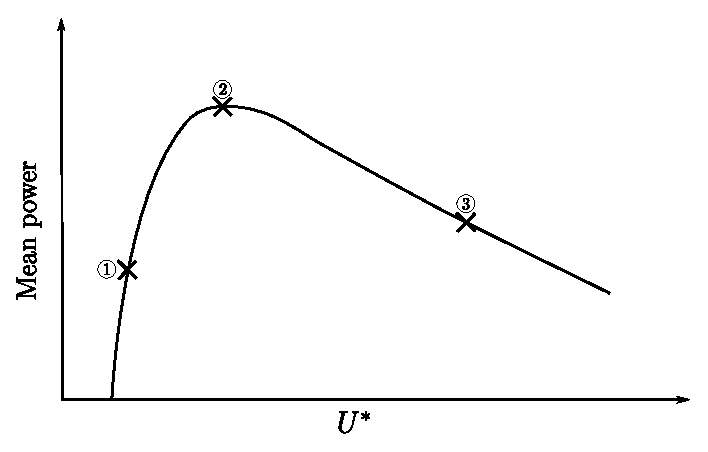
\includegraphics[width=0.5\textwidth]{../FnP/sketch_1}
\caption{ Three key regions taken into account to analyse the time histories of power in a typical mean power vs. $U^*$ curve at Re=165 }
\label{fig:regions_1}
\end{figure}


From Fig \ref{cy ploynomial} (a) shows that the instantaneous force rises until $4^0$ where it peaks and then falls and at round $6^0$ becomes negative. Maximum amount of power could be transferred within the peak region. At the region where the instantaneous force becomes negative it will be opposing the velocity $\dot{y}$.

$U^*=90$ (region 1) the damping constant is high and therefore a clear sinusoidal signal could be observed for both $P_d$ and $P_t$ Fig. \ref{fig:power_time_histories} (a). Fig.\ref{fig:power_time_histories} (d) and (g) shows that$\theta$ is in line or in phase with $F_y$. Hence both $P_d$ and $P_t$ becomes sinusoidal. However, due to the higher damping  $\theta$ does not go to the region where the peak power is produced.

At region 2 where the mean power output is at its maximum($U=165$), $P_t$ is not a pure sinusoidal signal. However, the  signal remains periodic. From the time history graph of $P_t$,two `peaks' are present in a single half cycle (Fig \ref{fig:power_time_histories} (b)). In this case at certain point in time $\theta$ arrives at the region where $F_y$ decreases but does not become negative when the angle is increased. Therefore, the force $F_y$ and $P_t$ reduces as the velocity further increases since $\theta = tan^{-1}(\frac{\dot{y}}{U})$. As the velocity $\dot{y}$ is sinusoidal, $\theta$ recovers back and this leads to two `peaks'  in a single half cycle.

At region 3 ($U^*= 400$) `$c$' is low in comparison with region 1 and 2 which leads to a low mean power output. From Fig.\ref{fig:power_time_histories} (c) .b $P_t$ becomes negative over some portion of the cycle. This is because $\theta$  passes the point where both $\theta$ and $c_y$ (therefore $c_y$) are positive. As the force opposes the direction of travel and the power becomes negative. On the other hand from an energy perspective we could see that the mechanical damping is not sufficient to dissipate out the energy transferred from the fluid to the structure during the part of the cycle when this occurs(as `$c$' is substantially low), therefore  part of this energy is transferred back to the fluid in the remaining part of the cycle.

 
  
\begin{figure}

  \setlength{\unitlength}{\textwidth}
%  \fbox{
  \begin{picture}(1,0.58)(0,0.35)
    % % % 90
    \put(0.03,0.76){\includegraphics[width=0.35\unitlength]{../FnP/gnuplot/power_time_history_90.eps}}
    \put(0.03,.58){\includegraphics[width=0.35\unitlength]{../FnP/gnuplot/f_y_history_90.eps}}
    \put(0.03,0.4){\includegraphics[width=0.35\unitlength]{../FnP/gnuplot/theta_time_history_90.eps}}
    
    % % 165
    \put(0.36,0.76){\includegraphics[width=0.35\unitlength]{../FnP/gnuplot/power_time_history_165.eps}}
    \put(0.36,.58){\includegraphics[width=0.35\unitlength]{../FnP/gnuplot/f_y_history_165.eps}}
    \put(0.36,0.4){\includegraphics[width=0.35\unitlength]{../FnP/gnuplot/theta_time_history_165.eps}}
    
    \put(0.68,0.76){\includegraphics[width=0.35\unitlength]{../FnP/gnuplot/power_time_history_400.eps}}
    \put(0.68,.58){\includegraphics[width=0.35\unitlength]{../FnP/gnuplot/f_y_history_400.eps}}
    \put(0.68,0.4){\includegraphics[width=0.35\unitlength]{../FnP/gnuplot/theta_time_history_400.eps}}
    
    \put(0.55,0.36){$\displaystyle{\frac{tU}{D}}$}
    \put(0.2,0.36){$\displaystyle{\frac{tU}{D}}$}
    \put(0.85,0.36){$\displaystyle{\frac{tU}{D}}$}
    
    \put(0.0,0.87){$\frac{P}{\rho \mathcal{A}U^3}$}
    \put(0.01,0.66){$F_y$}
    \put(0.01,0.49){$\theta$}
    
    \put(0.08,0.76){(a)}
    \put(0.08,0.58){(d)}
    \put(0.08,0.38){(g)}
    
    \put(0.4,0.76){(b)}
    \put(0.4,0.58){(e)}
    \put(0.4,0.38){(h)}
    
    \put(0.72,0.76){(c)}
    \put(0.72,0.58){(f)}
    \put(0.72,0.38){(i)}
  \end{picture}
%}
  \caption{Time histories of $P_t$, $P_d$, $F_y$ and $\theta$ at $\ustar=90$, $165$ and $400$ where the mean power dissipated due to mechanical damping was calculated using equation \hilight{equation}. Data was obtained at $\zeta=0.1$ and $m^*=40$. The time histories of $P_t$ ( \solidrule[4mm]\hspace{1mm}) and $P_d$ (\protect\dashedrule) are presented for: (a) $\ustar = 90$; (b) $\ustar = 165$; (c) $\ustar = 400$. Time histories of the instantaneous force $F_y$ for: (a) $\ustar = 90$; (b) $\ustar = 165$; (c) $\ustar = 400$. Time histories of the instantaneous angle $\theta$ for: (a) $\ustar = 90$; (b) $\ustar = 165$; (c) $\ustar = 400$.}
  \label{fig:power_time_histories}
\end{figure}





 



\subsection{Effect of $m^*$}

 \begin{figure}
\setlength{\unitlength}{\textwidth}

  \begin{picture}(1,0.35)(0,0.75)
    
  \put(0.15,0.76){\includegraphics[width=0.7\unitlength]{../FnP/gnuplot/mean_power_collapsed_mstar.eps}}         
      
      
   
 	\put(0.11,0.95){\large $\frac{P_{m}}{\rho \mathcal{A}U^3 }$} 	

 	
 	 	\put(0.45,0.75){ $c\rho\mathcal{A}U$} 	
 	 

     

  \end{picture}

  \caption{Mean power as a function of damping factor. Data are presented at $m^*=10$ (\ding{108}), $m^*=20$ (\ding{83}), $m^*=40$ (\ding{115}), $m^*=60$ (+) at Re 165 and $\zeta=0.1$. A reduction of maximum mean power can be observed when $m^*<40$. For $m^*>40$, the maximum power is essentially independent of $m^*$.}
    \label{fig:m_star_collapsed}
\end{figure}

The maximum mean power at different $m^*$ Fig.\ref{fig:m_star_collapsed} was constant beyond $m^*=30$. However, at $m^* \leq 30$ an effect of $m^*$ it could be observed that the mean power curve reduces with $m^*$. This may be due to the fact that as the inertia of the system is reduced.  

 
 
 This was also reported by \cite{Joly2012} where an influence of vortex shedding was present on galloping amplitude at low mass ratios. 



 \begin{figure}
  \setlength{\unitlength}{\textwidth}
  \begin{picture}(1,0.25)
    % % %90
    \put(0.02,0.03){\includegraphics[width=0.3\unitlength]{../FnP/gnuplot/fsi_displacement.eps}}
    \put(0.36,0.03){\includegraphics[width=0.3\unitlength]{../FnP/gnuplot/fsi_velocity.eps}}
    \put(0.72,0.03){\includegraphics[width=0.3\unitlength]{../FnP/gnuplot/fsi_power.eps}}
    
    \put(0.03,0.17){$\frac{A}{D}$}
    \put(0.36,0.17){$\frac{V}{D}$}
    \put(0.68,0.17){$\frac{P_{m}}{\rho \mathcal{A}U^3 }$}
    
    \put(0.18,0.0){\ustar} 	
    \put(0.51,0.0){\ustar}
    \put(0.87,0.0){\ustar}

    \put(0.092,0.21){\small(a)}
    \put(0.42,0.21){\small(b)}
    \put(0.78,0.21){\small(c)}

  \end{picture}  

  \caption{Comparison of data generated using the quasi-static theory (\ding{83}) and full DNS simulations (\ding{108}). (a) Displacement amplitude, (b) velocity amplitude and (c) mean power as functions of \ustar. Data were obtained at $Re=165$ and $\zeta=0.075$. An average difference of $34\%$ is observed for both displacement and velocity amplitude. However, the essential physics i.e the rise and fall of mean power, is captured by DNS simulations.}
    \label{fig:FSI_QSS_compare}
\end{figure}

\subsection{Comparsion with FSI simulations}
 Similar trends are captured for both displacement and velocity amplitudes between QSS and FSI simulations (Fig. \ref{fig:FSI_QSS_compare}(a) and \ref{fig:FSI_QSS_compare}(b)). Quantitatively a large discrepancy (average of $30\%$) could be observed between QSS and FSI data. Therefore the power also becomes significantly low (Fig.\ref{fig:FSI_QSS_compare}(c)). However, the FSI data (Fig.\ref{fig:FSI_QSS_compare} (c)) was able to produce the main the rise and the fall of mean power as $U^*$ is increased. The reasoning behind this the fact is that galloping is weak at Re 165  and therefore fluid damping has a significant effect. It was reported by \cite{Barrero-Gil2009} that galloping only starts to occur ar Re $\geq 159$. As power is function of $(\dot{y})^2$ the error between QSS and FSI power becomes significantly large.  
 
 Put conclusion here 
 
 

%\section{Conclusion}









 

 
 
 

 
 


 % % % % % % % % % % % % % % % % % % % % % % % % % % % % % % % % % % % % % % % % %

 
 
 
 
 
 
 
 
 
 
  
 
 
%\begin{figure}
  \setlength{\unitlength}{\textwidth}

  \begin{picture}(1,1.13)(0,0)
    
    % % %90
      \put(0.25,0.78){\includegraphics[width=0.5\unitlength]{../FnP/gnuplot/fsi_displacement.eps}}
      \put(0.25,0.4){\includegraphics[width=0.5\unitlength]{../FnP/gnuplot/fsi_velocity.eps}}
      \put(0.25,0.025){\includegraphics[width=0.5\unitlength]{../FnP/gnuplot/fsi_power.eps}}
     
   
	
            
      
      
   
 	\put(0.25,0.98){ \large $\frac{A}{D}$} 	
 	\put(0.25,0.62){\large $\frac{V}{D}$}
 	\put(0.2,0.23){\large $\frac{P_{m}}{\rho \mathcal{A}U^3 }$}
 	
% 	 	\put(0.25,0.88){ \ustar} 	
% 	 	\put(0.8,0.88){ \ustar}
 	 	\put(0.5,0.0){ \ustar}



    \put(0.36,1.1){(a)}
    \put(0.34,0.72){(b)}
    \put(0.34,0.34){(c)}
   
       

  \end{picture}  
	
  \caption{Comparison of QSS (\ding{83}) and FSI (\ding{108}) data of displacement amplitude, velocity amplitude and mean power as a function of \ustar represented by (a), (b) and (c)respectively. Data were obtained at Re=165 and $\zeta=0.075$. An average error of $34\%$ could be observed for both displacement and velocity amplitude. Essential physics i.e the rise and fall of mean power could be captured of the FSI data}
    \label{fig:FSI_QSS_compare}
\end{figure}

%% The Appendices part is started with the command \appendix;
%% appendix sections are then done as normal sections
%% \appendix

%% \section{}
%% \label{}

%% References
%%
%% Following citation commands can be used in the body text:
%%
%%  \citet{key}  ==>>  Jones et al. (1990)
%%  \citep{key}  ==>>  (Jones et al., 1990)
%%
%% Multiple citations as normal:
%% \citep{key1,key2}         ==>> (Jones et al., 1990; Smith, 1989)
%%                            or  (Jones et al., 1990, 1991)
%%                            or  (Jones et al., 1990a,b)
%% \cite{key} is the equivalent of \citet{key} in author-year mode
%%
%% Full author lists may be forced with \citet* or \citep*, e.g.
%%   \citep*{key}            ==>> (Jones, Baker, and Williams, 1990)
%%
%% Optional notes as:
%%   \citep[chap. 2]{key}    ==>> (Jones et al., 1990, chap. 2)
%%   \citep[e.g.,][]{key}    ==>> (e.g., Jones et al., 1990)
%%   \citep[see][pg. 34]{key}==>> (see Jones et al., 1990, pg. 34)
%%  (Note: in standard LaTeX, only one note is allowed, after the ref.
%%   Here, one note is like the standard, two make pre- and post-notes.)
%%
%%   \citealt{key}          ==>> Jones et al. 1990
%%   \citealt*{key}         ==>> Jones, Baker, and Williams 1990
%%   \citealp{key}          ==>> Jones et al., 1990
%%   \citealp*{key}         ==>> Jones, Baker, and Williams, 1990
%%
%% Additional citation possibilities
%%   \citeauthor{key}       ==>> Jones et al.
%%   \citeauthor*{key}      ==>> Jones, Baker, and Williams
%%   \citeyear{key}         ==>> 1990
%%   \citeyearpar{key}      ==>> (1990)
%%   \citetext{priv. comm.} ==>> (priv. comm.)
%%   \citenum{key}          ==>> 11 [non-superscripted]
%% Note: full author lists depends on whether the bib style supports them;
%%       if not, the abbreviated list is printed even when full requested.
%%
%% For names like della Robbia at the start of a sentence, use
%%   \Citet{dRob98}         ==>> Della Robbia (1998)
%%   \Citep{dRob98}         ==>> (Della Robbia, 1998)
%%   \Citeauthor{dRob98}    ==>> Della Robbia


%% References with bibTeX database:

\clearpage

\bibliographystyle{elsarticle-harv}
\bibliography{../../BibteX/Paper}

%% Authors are advised to submit their bibtex database files. They are
%% requested to list a bibtex style file in the manuscript if they do
%% not want to use elsarticle-harv.bst.

%% References without bibTeX database:

% \begin{thebibliography}{00}

%% \bibitem must have one of the following forms:
%%   \bibitem[Jones et al.(1990)]{key}...
%%   \bibitem[Jones et al.(1990)Jones, Baker, and Williams]{key}...
%%   \bibitem[Jones et al., 1990]{key}...
%%   \bibitem[\protect\citeauthoryear{Jones, Baker, and Williams}{Jones
%%       et al.}{1990}]{key}...
%%   \bibitem[\protect\citeauthoryear{Jones et al.}{1990}]{key}...
%%   \bibitem[\protect\astroncite{Jones et al.}{1990}]{key}...
%%   \bibitem[\protect\citename{Jones et al., }1990]{key}...
%%   \harvarditem[Jones et al.]{Jones, Baker, and Williams}{1990}{key}...
%%

% \bibitem[ ()]{}

% \end{thebibliography}

\end{document}

%%
%% End of file `elsarticle-template-harv.tex'.
